\chapter{Arquitectura del sistema}
\section{Diseño general del sistema}

Descripción en prosa del diseño del sistema. Resalte cualquier detalle que considere de importancia para la comprensión del diseño. Indique cuál patrón arquitectónico está utilizando como base para su sistema. Si está utilizando un \textit{framework} para apoyar el proceso de desarrollo, descríbalo en esta sección. Cite y referencie adecuadamente la información que lo requiera.
]

La aplicación está construida sobre el framework Electron, lo que influencia en gran medida la arquitectura del sistema. Una aplicación en Electron tiene un proceso de ejecución principal que corre Node.js, este se encarga de la comunicación con el sistema operativo, la creación de ventanas, entre otras cosas; utilizando las bibliotecas que provee Electron. El proceso principal a su vez puede crear uno o más procesos renderizadores (renderer process), cada uno con una ventana asignada, estos procesos corren un navegador Chromium que se encarga de desplegar la interfaz de la aplicación (aunque también puede realizar más tareas con scripts de javascript). Esto provoca que la arquitectura este dividida en 2 partes: el proceso principal y el renderer. 

En esta aplicación el renderer es el encargado de desplegar la interfaz de usuario principal donde se  visualizan los documentos pdf y los botones, y demás elementos, usados para las otras funcionalidades del sistema. El proceso principal se encarga de la creación de ventanas del sistema (como la ventana principal, diálogos del sistema, menú contextual, etc), la comunicación con el sistema operativo, las funcionalidades que modifican los documentos y cuenta con el estado de la aplicación.

El código del proyecto tiene un diseño modular basado en los módulos de javascript. En cada módulo se encuentran funciones exportadas (públicas) y las funciones no exportadas (privadas) que solo se utilizan a lo interno del módulo. Cada módulo es responsable de una funcionalidad del sistema. Usualmente un módulo del proceso principal tiene una versión análoga en el renderer.

IPC

\subsection{Diagrama de dependencias}

El diagrama de dependencias muestra las dependencias entre los módulos de la aplicación. Es una forma útil de visualizar como trabajan los módulos de la aplicación entre sí y de que forma se relacionan. Este diagrama es generado utilizando la herramienta madge, así que muestra el proyecto tal y como está programado. También, puede resultar útil para detectar dependencias circulares o un flujo extraño dentro del programa.

El formato del diagrama es el siguiente. Cada archivo o módulo del sistema es un rectángulo, el color representa el estado de la dependencia: azul si tiene dependencias, verde si no tiene dependencias y rojo si es parte de una dependencia circular. Las flechas indican las dependencias entre módulos.

\subsubsection{Proceso principal}

\begin{figure}[H]
	\centering
	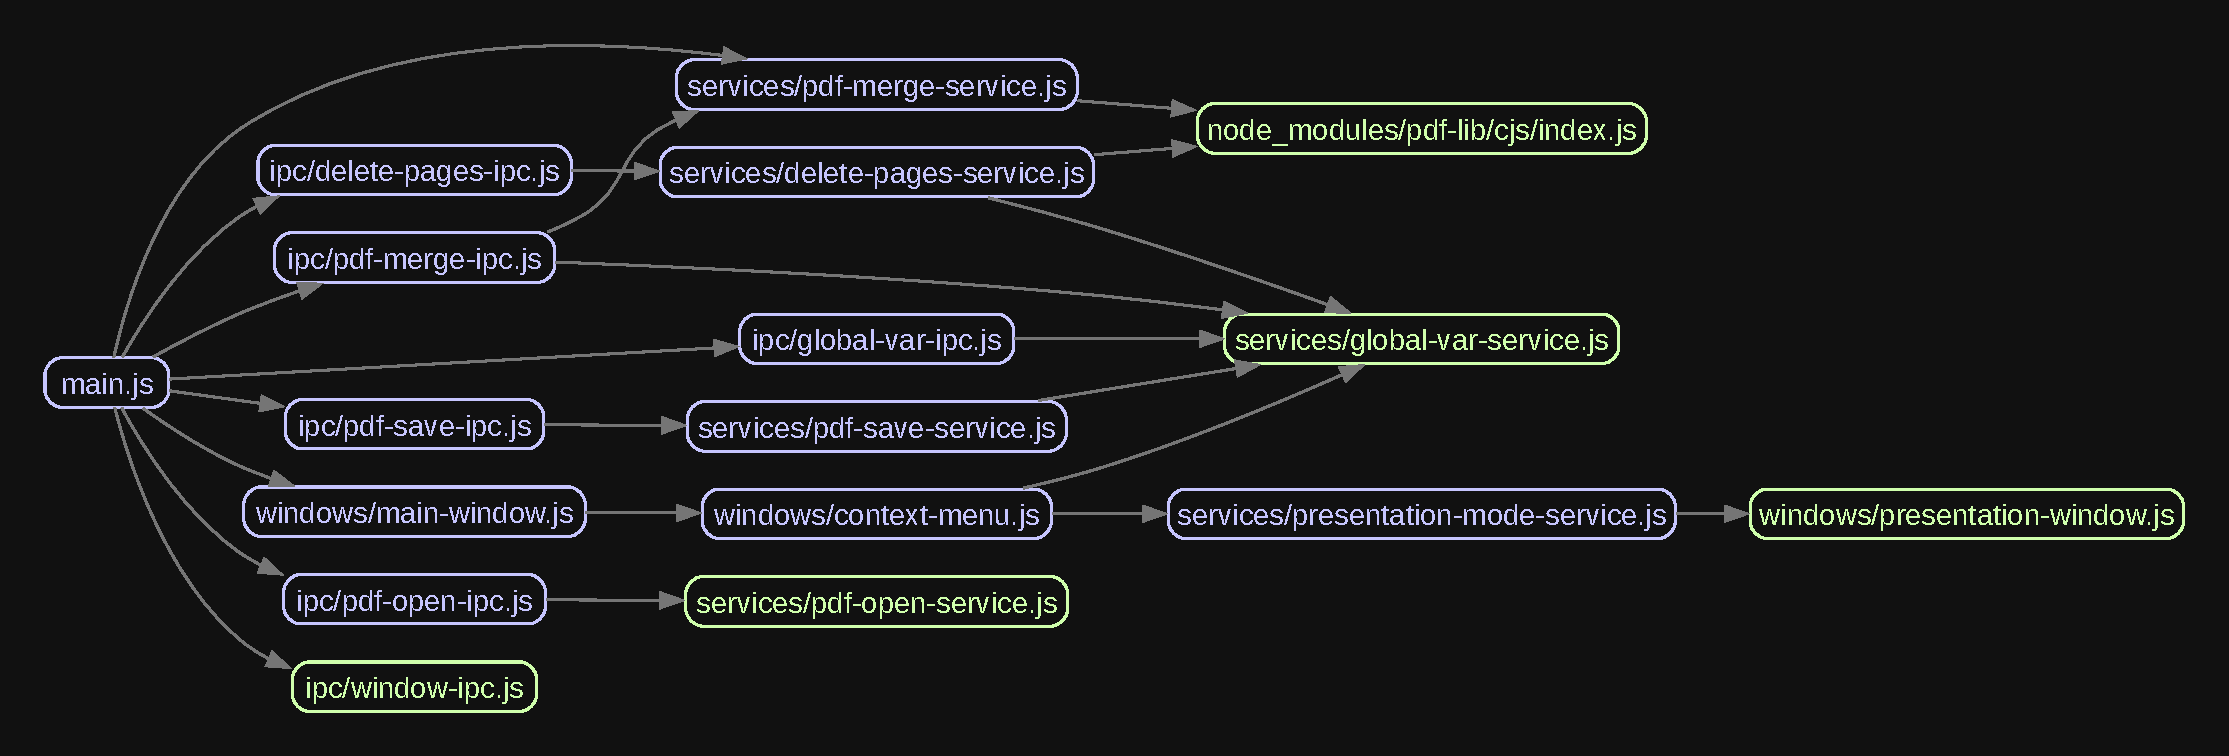
\includegraphics[width=\linewidth]{project/images/dd_main.pdf}
	\caption{\textbf{Diagrama de Dependecias: proceso principal}}
	\label{DiagramaDependenciaMain}
\end{figure}

\subsubsection{Proceso renderer}

\begin{figure}[H]
	\centering
	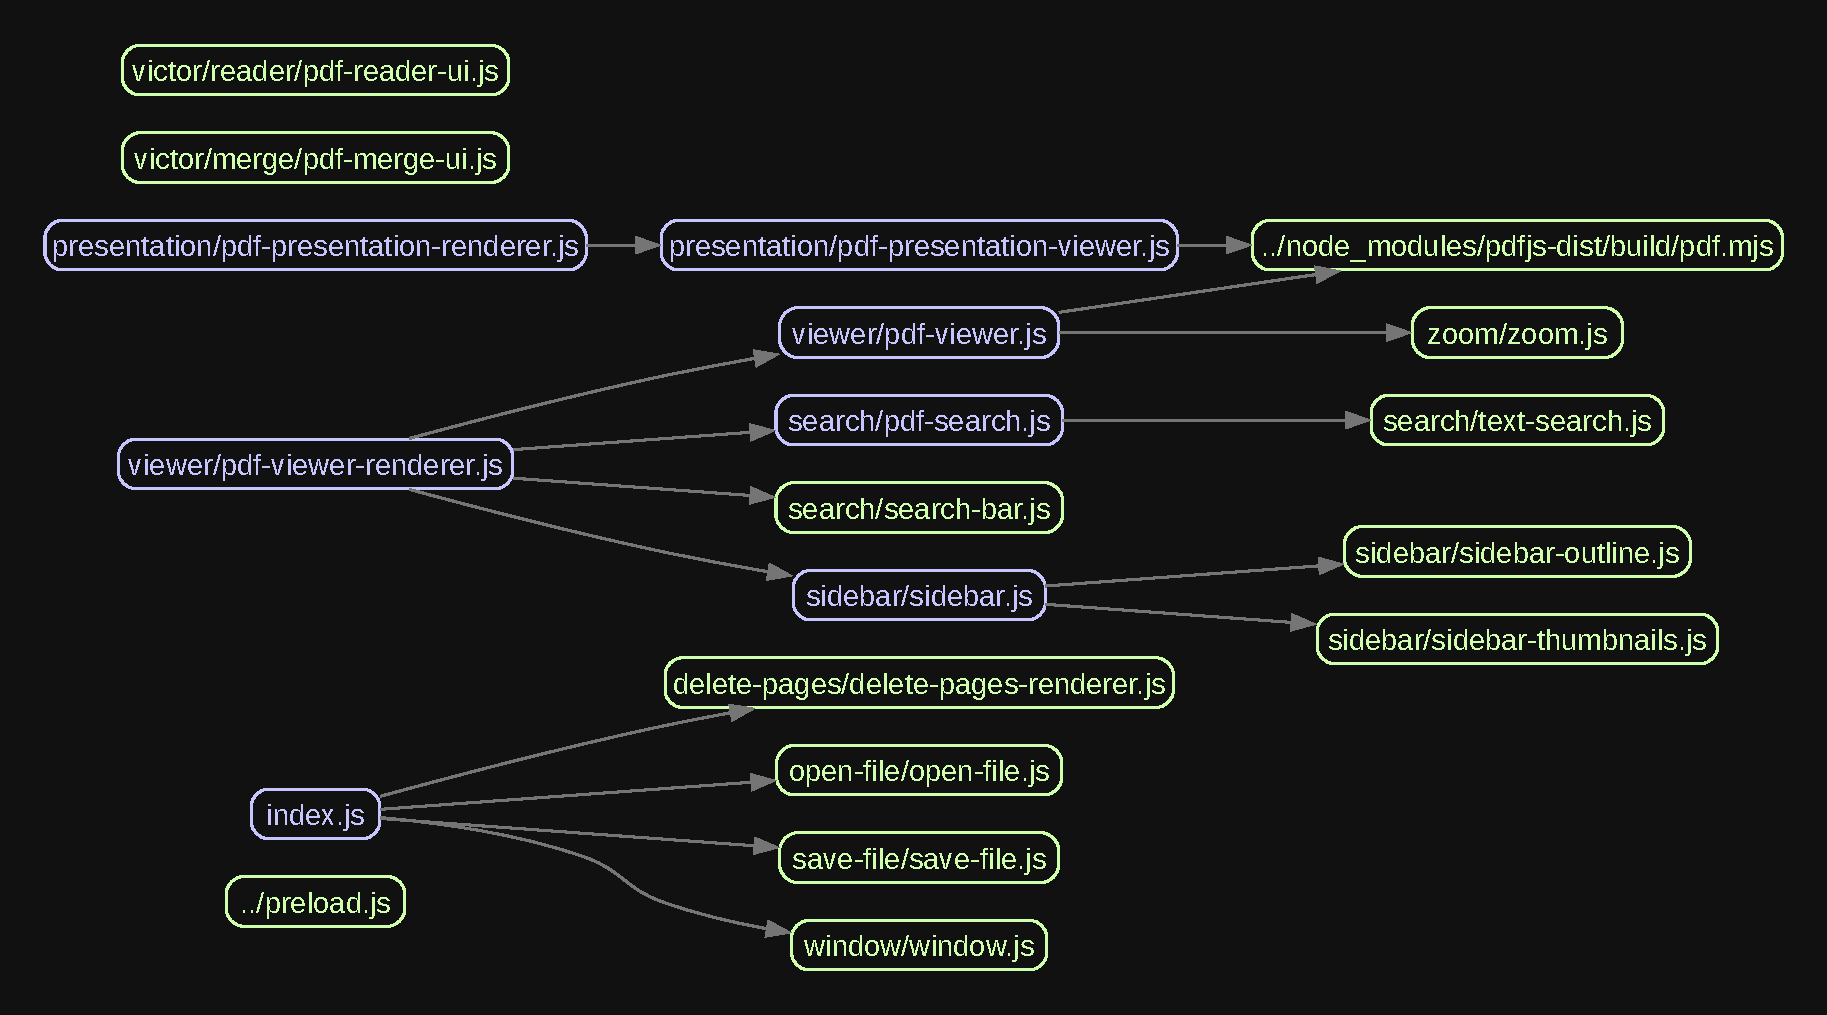
\includegraphics[width=\linewidth]{project/images/dd_renderer.pdf}
	\caption{\textbf{Diagrama de Dependecias: proceso renderer}}
	\label{DiagramaDependenciaRenderer}
\end{figure}



\subsection{Diseño de la persistencia}
Describa en esta sección la estrategia que abordó para diseñar la persistencia del sistema, incluya un diagrama para el modelo conceptual (Entidad-Relación) del sistema. Especifique cuáles aspectos del diseño fue necesario cambiar desde la última iteración, justifique todos los cambios.

\begin{figure}[H]
  \centering
    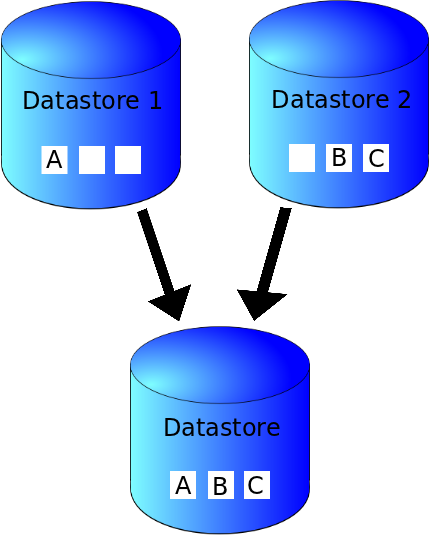
\includegraphics[height= 10cm, width=15cm]{project/images/data-sync}
  \caption{\textbf{IMAGE CAPTION}}
\end{figure}

Incluya y describa el modelo lógico (Diagrama relacional) de su sistema. Especifique todos los aspectos del diseño que fue necesario cambiar desde la última iteración, justifique todos los cambios.

\begin{figure}[H]
  \centering
    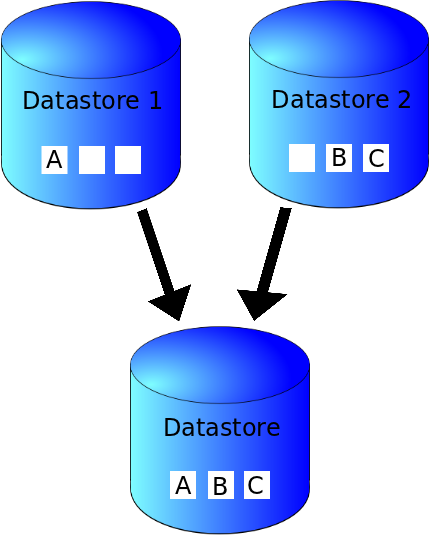
\includegraphics[height= 10cm, width=15cm]{project/images/data-sync}
  \caption{\textbf{IMAGE CAPTION}}
\end{figure}
	
\subsection{Diagrama de clases}
Añada una imagen con el diagrama de clases del sistema,  preferiblemente desarrollado en DIA. Introdúzcala con un párrafo breve que enlace el diagrama con la descripción en prosa del encabezado de sección. Se recomienda que el diagrama se diseñe de forma que calce bien en una página vertical, de forma que se facilite su lectura. Recuerde hacer referencia a su diagrama de clases usando la referencia correcta. Por ejemplo, en la Figura \ref{DiagramaClases} se encuentra el diagrama de clases.
\begin{figure}[H]
  \centering
    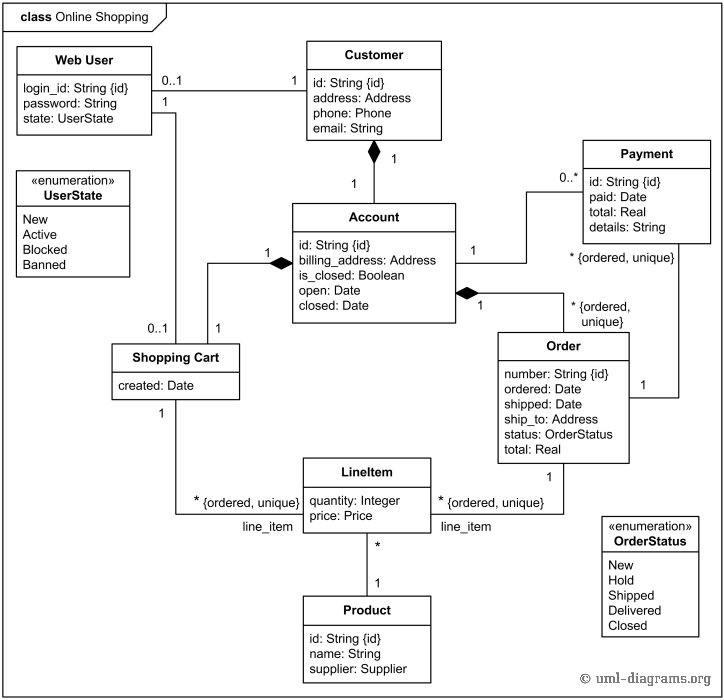
\includegraphics[ width=15cm]{project/images/class-example-online-shopping-domain.png}
  \caption{\textbf{IMAGE CAPTION}}
  \label{DiagramaClases}
\end{figure}


